\documentclass[aspectratio=169,11pt]{beamer}
\usetheme{Madrid}
\usepackage[T1]{fontenc}
\usepackage{tikz}
\usetikzlibrary{arrows.meta,positioning,calc}
\usepackage{amssymb}
\usepackage{listings}
\usepackage{booktabs}
\usepackage{array}
\lstset{basicstyle=\ttfamily\fontsize{8}{9.4}\selectfont,breaklines=true,breakindent=8pt,columns=fullflexible,keepspaces=true,showstringspaces=false,upquote=false,literate={~}{{\textasciitilde}}1}
\newcommand{\code}[1]{\texttt{\detokenize{#1}}}
% PRINCIPLE tag: consistent orange box in the title bar, top right
\newcommand{\princ}[1]{\begin{tikzpicture}[remember picture,overlay]\node[anchor=north east,fill=orange!85!red,text=white,font=\bfseries\fontsize{7}{8}\selectfont,inner sep=3pt,text width=6.2cm,align=center,rounded corners=2pt] at ([xshift=-5pt,yshift=-5pt]current page.north east){\hyphenpenalty=10000\relax PRINCIPLE: #1};\end{tikzpicture}}
% PROMPT FOR CLAUDE box: text comes from prompts_txt/ (copied from the real prompt files)
\newcommand{\promptbox}[2]{\IfFileExists{prompts_txt/#1_#2.txt}{\begin{alertblock}{PROMPT FOR CLAUDE \hfill {\scriptsize prompts/\input{prompts_txt/#1.name}}}\lstinputlisting{prompts_txt/#1_#2.txt}\end{alertblock}}{\begin{alertblock}{PROMPT FOR CLAUDE (#1 #2)}PENDING: prompt file not copied yet.\end{alertblock}}}
\newcommand{\see}[1]{{\small\textbf{\textcolor{green!40!black}{What you should see:}} #1\par}}
\newcommand{\recover}[1]{{\scriptsize\textbf{Recovery:} #1\par}}
\newcommand{\predict}[1]{{\small\textbf{\textcolor{blue!60!black}{1 PREDICT (30 s):}} #1\par}}
\newcommand{\mistake}[1]{{\scriptsize\textbf{\textcolor{red!60!black}{Common mistake:}} #1\par}}
\newcommand{\badge}[2]{\colorbox{#1}{\textcolor{white}{\textbf{\footnotesize\ #2\ }}}}
\newcommand{\redbadge}[1]{\badge{red!70!black}{STEP #1 \textbullet\ RED}}
\newcommand{\greenbadge}[1]{\badge{green!45!black}{STEP #1 \textbullet\ GREEN}}
\newcommand{\loopstrip}{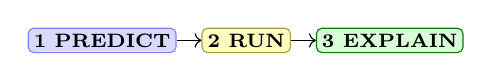
\begin{tikzpicture}[baseline=-0.5ex,font=\scriptsize\bfseries,node distance=9pt]\node[fill=blue!15,draw=blue!50,rounded corners=2pt,inner sep=2pt](a){1 PREDICT};\node[fill=yellow!25,draw=yellow!60!black,rounded corners=2pt,inner sep=2pt,right=of a](b){2 RUN};\node[fill=green!15,draw=green!50!black,rounded corners=2pt,inner sep=2pt,right=of b](c){3 EXPLAIN};\draw[->](a)--(b);\draw[->](b)--(c);\end{tikzpicture}}
\title{Relations in Your Tests}
\subtitle{From idea to proposal to plan to working, tested code}
\author[COMSC 2043 DSCT]{COMSC 2043 \textbullet\ Discrete Structures and Critical Thinking}
\date{Week 11, October 27, 2026}
